The second independent replication was done with the extended algorithms (AL, SAL and LAL) previously presented in Section \ref{sec:changes}. The assessment was done in the same dynamic context used by the first replication (see Section \ref{sec:original}), following similar original algorithms conditions and variables values.

Table \ref{table:table02} shows the total reward obtained with the completed tasks, elapsed time to perform the tasks, number of completed tasks, the quality obtained with the completed tasks and the total number of tokens sent. These results were obtained applying the independent variables of 100 executions, 96 tasks, 9 UAVs and the same \textit{stimulus} and sensors quality used by the original experiments.

\begin{table}%[ht]
	\small
	\fontsize{6}{6}\selectfont
	\centering
	\caption{Total reward, elapsed time, quantity and quality of the completed tasks and number of exchanged messages for 100 runs of each algorithm after modification, described in Section \ref{sec:changes}, with the following attributes: 9 UAVs and 96 tasks in area of 300x240 pixels with deadline of 300 ticks.}
	\label{table:table02}
	
	\begin{tabular}{rrrrr} \hline
		& AL
		& SAL
		& LAL \\ \hline 
		
		& Mean (St.Dev.)  & Mean (St.Dev.)  & Mean (St.Dev.)  \\ [1ex]
		
		\multicolumn{5}{l}{\textbf{Results obtained with the algorithms after modifications described in Section \ref{sec:dynamic_scenario}}} \\
	Total reward           & 4.9713   ($\pm$1.4175)  & 15.6611  ($\pm$1.7195) & 18.2397 ($\pm$1.8068)   \\
	Elapsed time (norm)    & 0.9355   ($\pm$0.0683)  &  0.9143  ($\pm$0.0534) & 0.9067  ($\pm$0.0643)    \\ 
	Comp. tasks (norm)     & 0.0773   ($\pm$0.0175)  &  0.1741  ($\pm$0.0182) & 0.1993  ($\pm$0.0193)    \\ 
	Quality (norm)         & 0.7932   ($\pm$0.1053)  &  0.9980  ($\pm$0.0083) & 0.9993  ($\pm$0.0040)   \\ 
	Sending token          & 47.9600  ($\pm$1.9012)  &  48.0200 ($\pm$2.0100) & 148.6200($\pm$4.8550)   \\ [1ex]
	
		\hline
	\end{tabular}
\end{table} 


The results obtained by these modified algorithms, with small number of UAVs(3) and tasks (4, 8 and 16), presented less difference from the original algorithms in the dynamic scenario (Section \ref{sec:original}). As the number of elements is low, the differences are within the standard deviation. Therefore, the largest group (9 UAVs and 96 tasks) was used to emphasize the variation values. Table \ref{table:table03} shows the results of quality and number of exchanged messages obtained by this replication, but with fewer UAVs and a different number of tasks.

\begin{table}%[ht]
	\small
	\fontsize{6}{6}\selectfont
	\centering
	\caption{Quality and number of exchanged messages of the customized algorithms}
	\label{table:table03}
	
	\begin{tabular}{rrrrr} \hline
		& AL
		& SAL
		& LAL \\ \hline 
		
		& Mean (St.Dev.)  & Mean (St.Dev.)  & Mean (St.Dev.)  \\ [1ex]
		
		\multicolumn{5}{l}{\textbf{3 UAVs and 4 tasks in area of 100x80 pixels with deadline of 300 ticks}} \\
	Quality (norm)         & 0.8218   ($\pm$0.1747)  &  0.8437  ($\pm$0.1434) & 0.9215  ($\pm$0.1115)   \\ 
	Sending token          &  5.0800  ($\pm$2.3471)  &  5.3000  ($\pm$2.8972) & 7.0300  ($\pm$2.3632)   \\ [1ex]
		
		\multicolumn{5}{l}{\textbf{3 UAVs and 8 tasks in area of 100x80 pixels with deadline of 300 ticks}} \\
	Quality (norm)         & 0.7151  ($\pm$0.1218)  & 0.7494  ($\pm$0.1399) &  0.8047  ($\pm$0.0978)  \\ 
	Sending token          & 10.6100 ($\pm$2.5222)  & 10.1900 ($\pm$2.9566) &  14.7600 ($\pm$2.8467)  \\ [1ex]
	
	    \multicolumn{5}{l}{\textbf{3 UAVs and 16 tasks in area of 100x80 pixels with deadline of 300 ticks}} \\
	Quality (norm)         & 0.7505  ($\pm$0.1290)  & 0.8813  ($\pm$0.0902) &  0.9532  ($\pm$0.0505)  \\ 
	Sending token          & 9.7600  ($\pm$2.4000)  & 10.1700 ($\pm$2.2699) &  25.7400 ($\pm$3.4160)  \\ [1ex]
	
	    \multicolumn{5}{l}{\textbf{3 UAVs and 32 tasks in area of 100x80 pixels with deadline of 300 ticks}} \\
	Quality (norm)         & 0.7134  ($\pm$0.1094)  & 0.9502  ($\pm$0.0479) &  0.9742  ($\pm$0.0269)  \\ 
	Sending token          & 6.8900  ($\pm$1.1712)  & 7.0600  ($\pm$1.2045) &  32.1500 ($\pm$1.8607)  \\ [1ex]
	
	    \multicolumn{5}{l}{\textbf{6 UAVs and 64 tasks in area of 200x160 pixels with deadline of 300 ticks}} \\
	Quality (norm)         & 0.7834  ($\pm$0.1374)  & 0.9919  ($\pm$0.0185) &  0.9968  ($\pm$0.0127)  \\ 
	Sending token          & 22.4000 ($\pm$1.3559)  & 22.1300 ($\pm$1.3154) &  95.2100 ($\pm$3.5142)  \\ [1ex]

		\hline
	\end{tabular}
\end{table} 






Overall, the data from Table \ref{table:table03} show that after the modifications described in Section \ref{sec:changes}, resulting in extended algorithms, different results were obtained  compared with the original ones in the dynamic scenario. From all assessed metrics, quality and number of exchanged messages were those with more significant variation.

In particular, the number of messages increases over 100\% with the modified algorithms, indicating a communication overhead. The exchanged messages in the original and the modified algorithms are depicted in Figure \ref{fig:fig06}.

\begin{figure}[h!]
	\begin{center}
		%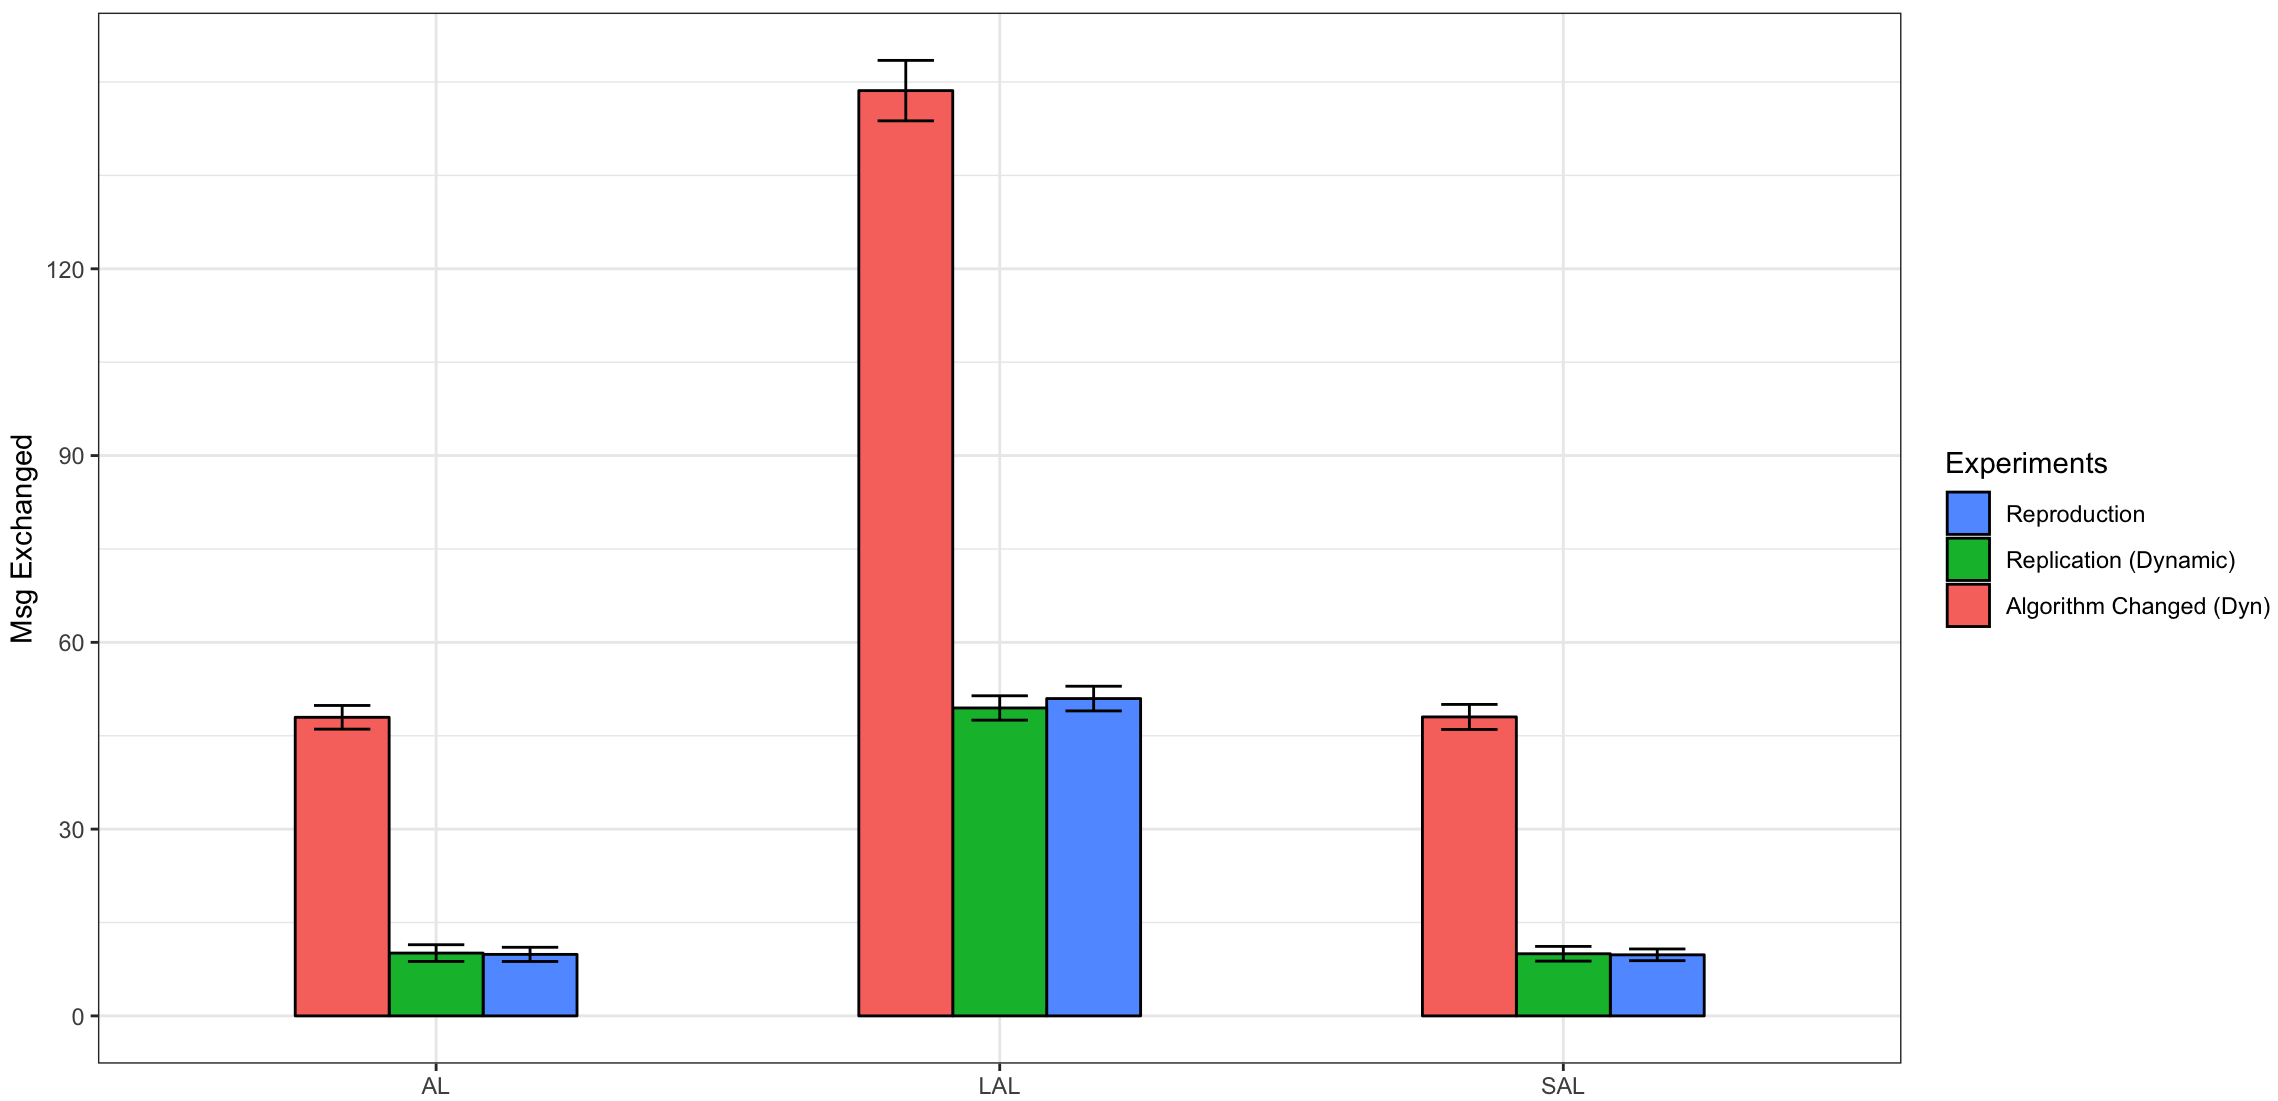
\includegraphics[scale=0.15]{fig/fig06.png}
		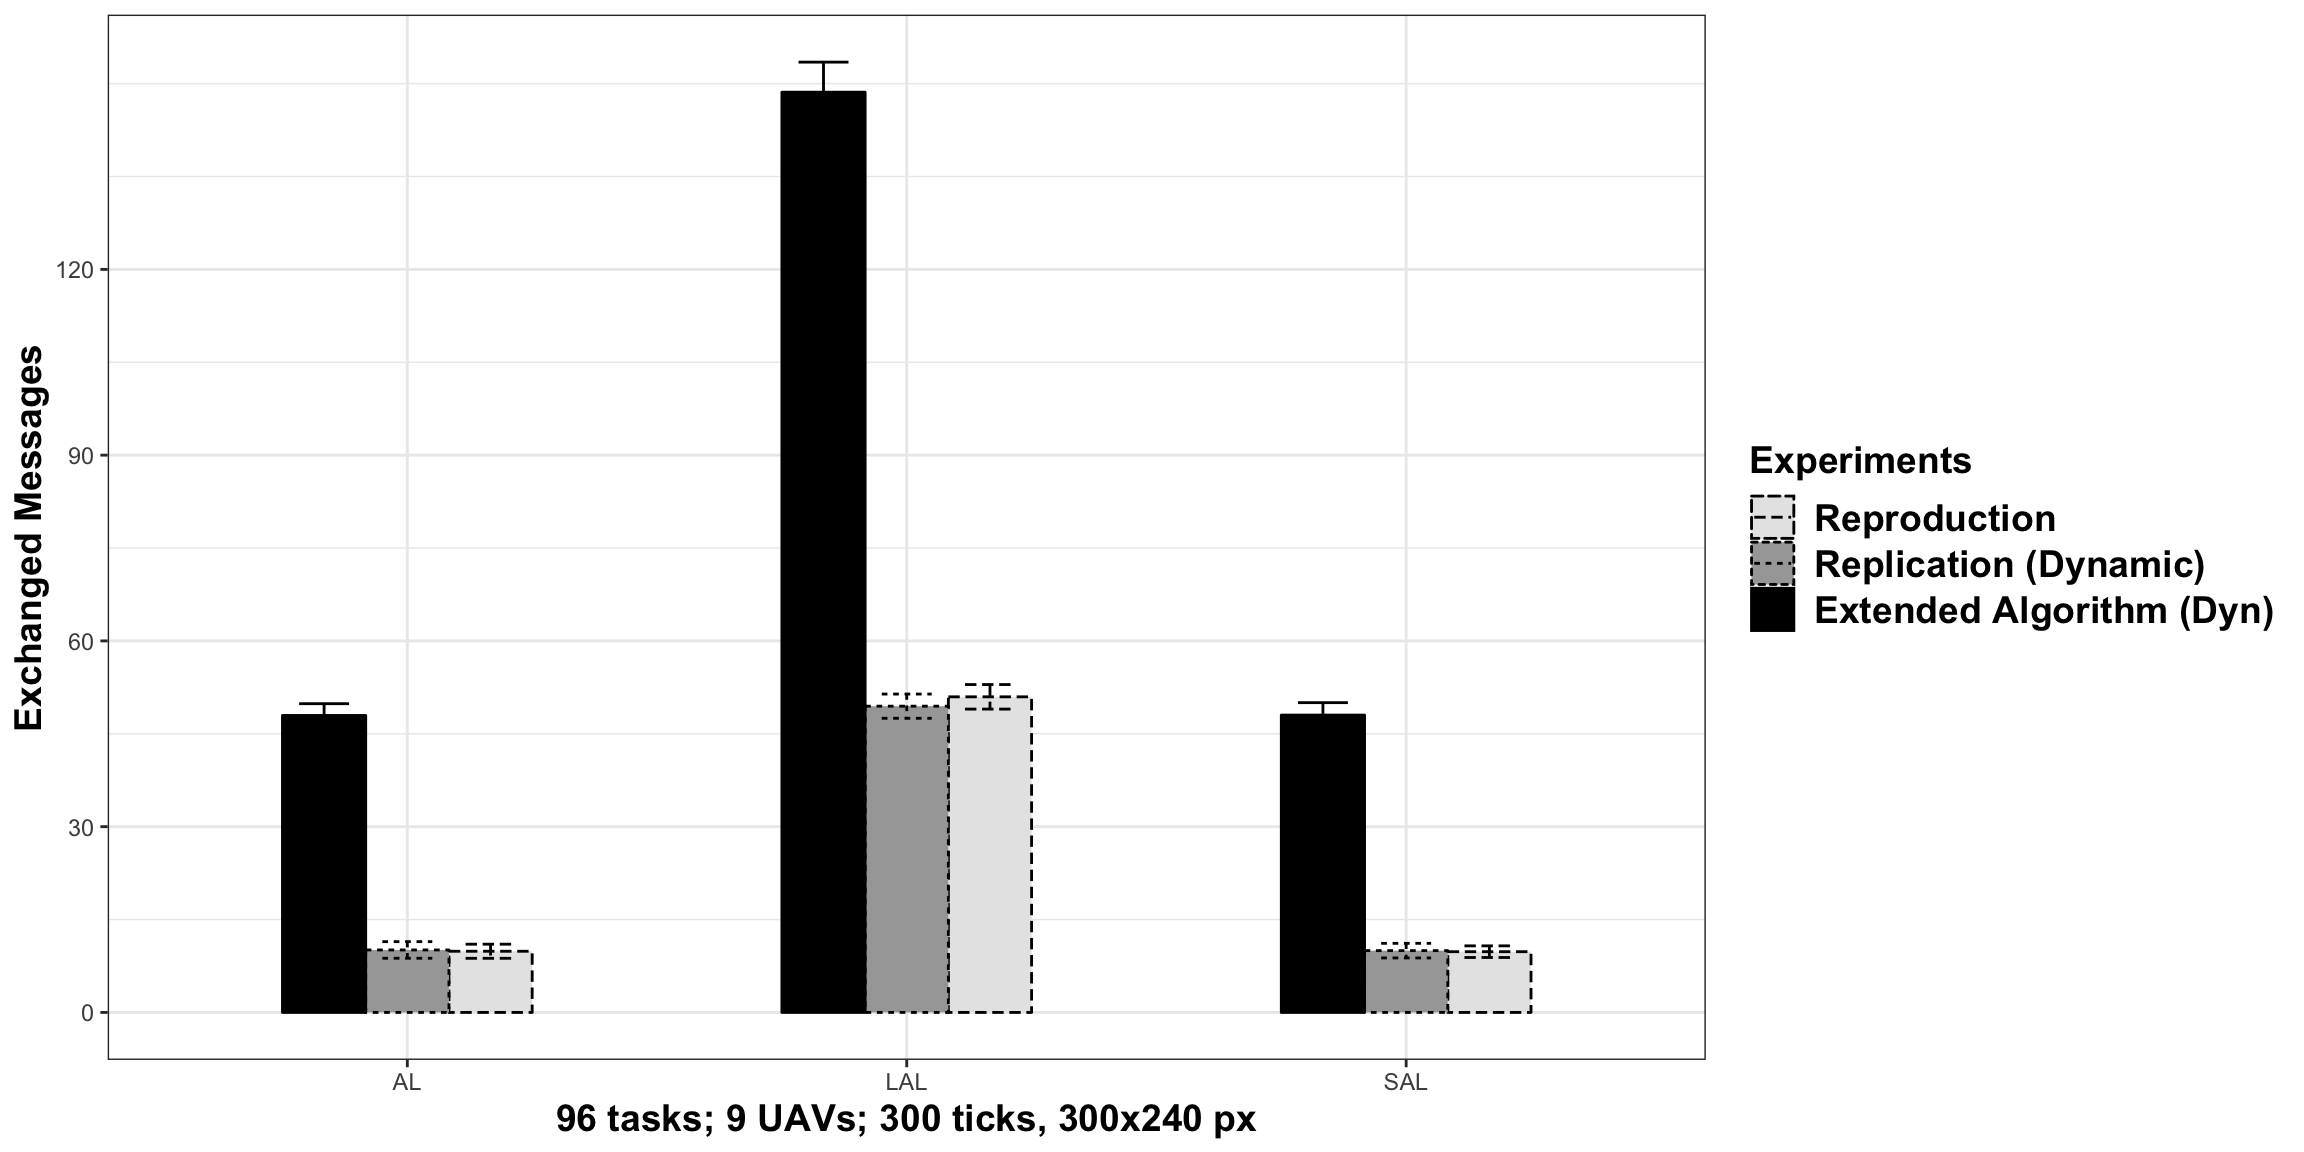
\includegraphics[scale=0.15]{fig/GRAPH06.png}
		\caption{Exchanged messages  of the original algorithm in the static scenario (reproduction), in the dynamic scenario (replication) and the modified algorithms in dynamic scenario (96 tasks; 9 UAVs; 300 x 240; 300 ticks)}
		\label{fig:fig06}
	\end{center}
\end{figure}

This overhead can be explained by the token reset made in the modified algorithms (see Line \ref{line:step2_begin} in Algorithm \ref{algo:change}). Resetting the token allows it to run more often among the UAVs, generating more messages exchanged among these elements.

Figure \ref{fig:fig05} shows that the extended algorithms presented an increase of around 40\% in the quality attribute compared with what was obtained in the first replication (Section \ref{sec:original}). This recovering was due to the task redistribution with the token reset after a context change with a UAV removed from the team. The new token round through the UAVs ensures reallocating tasks to maximize the quality results, relating the task with the agent that has the best sensor to perform it.

\begin{figure}[h!]
	\begin{center}
		%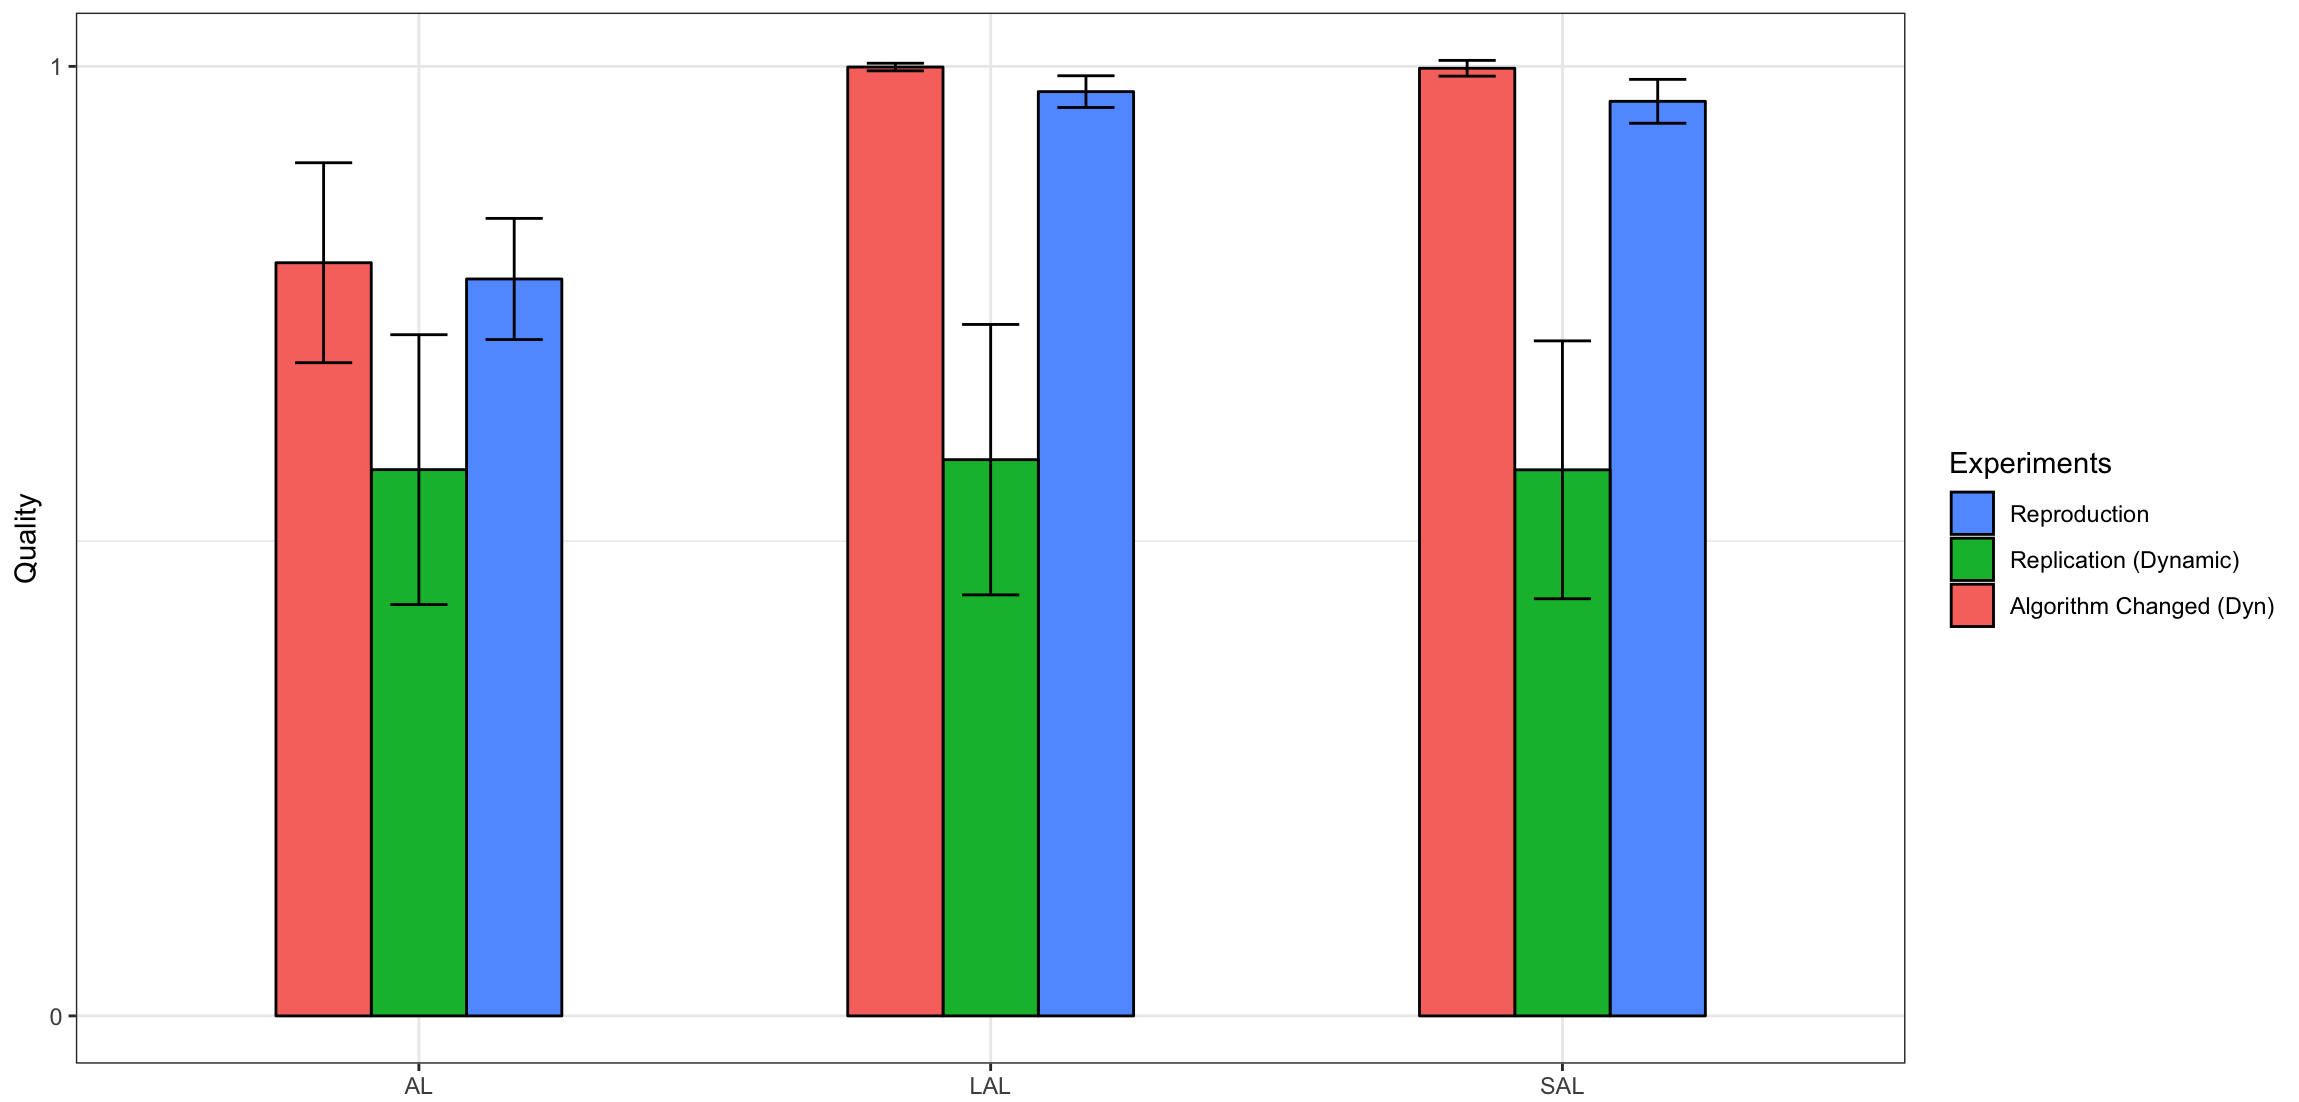
\includegraphics[scale=0.15]{fig/fig05.png}
		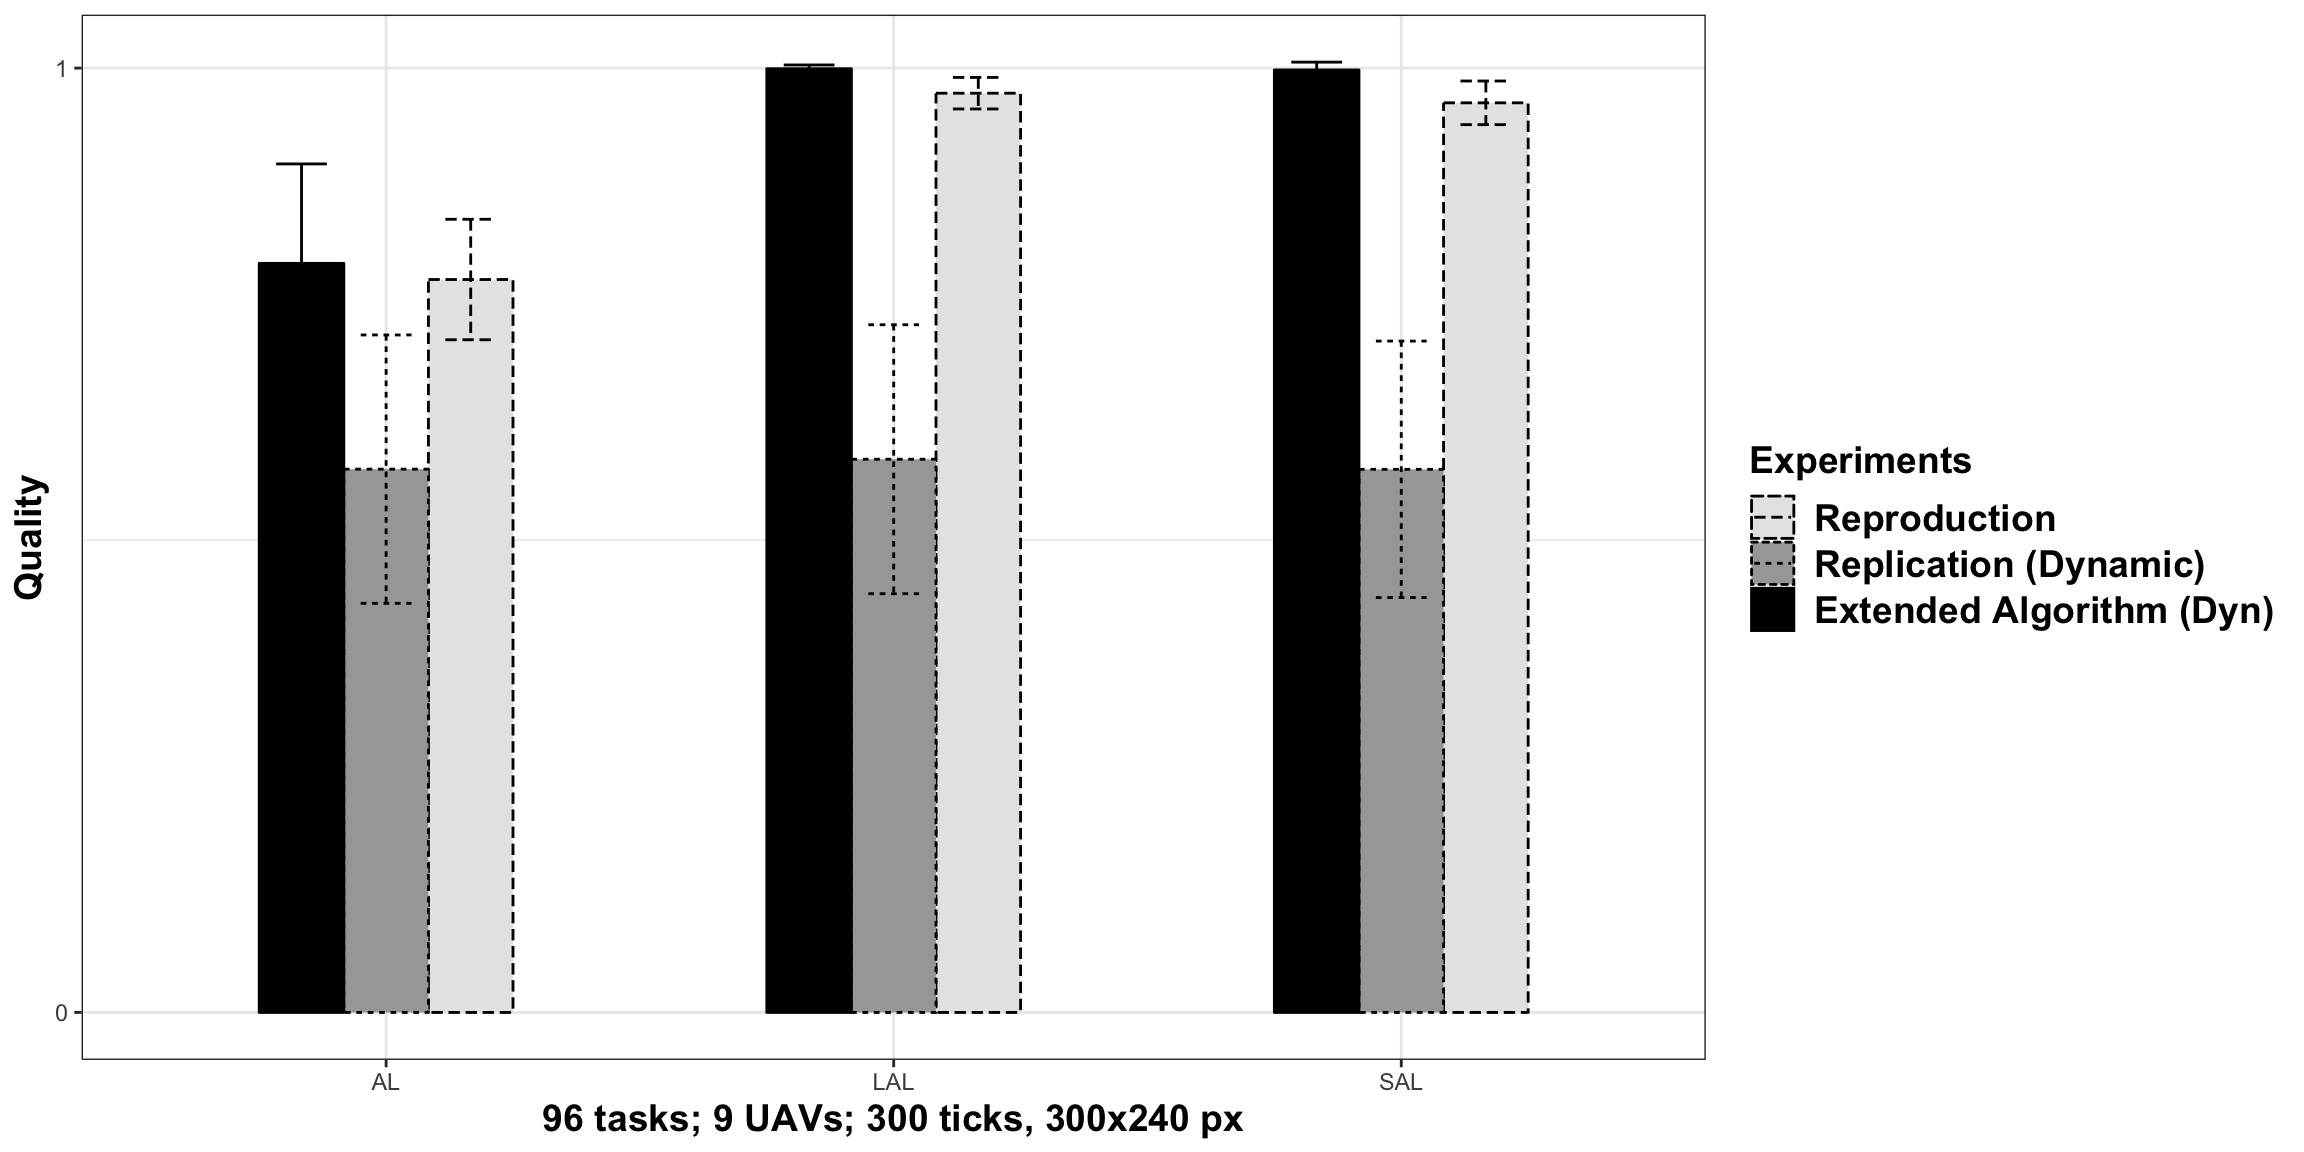
\includegraphics[scale=0.15]{fig/GRAPH07.png}
		\caption{Quality of the original algorithm in the static scenario (reproduction), in the dynamic scenario (replication) and the modified algorithms in dynamic scenario (96 tasks; 9 UAVs; 300 x 240; 300 ticks)}
		\label{fig:fig05}
	\end{center}
\end{figure}

 Figure \ref{fig:din02} shows the elapsed time to perform all tasks allocated to the UAVs. It presented a slight decrease of around 5\% because the agents spend more time communicating and adjusting the tasks allocation in order to optimize the quality. It results in less time available to execute the tasks due to the reallocation. However, the difference among the three algorithms (AL, SAL and LAL) in the dynamic context is within the standard deviation as seen in Figure \ref{fig:din02}.
 
\begin{figure}[h!]
	\begin{center}
		%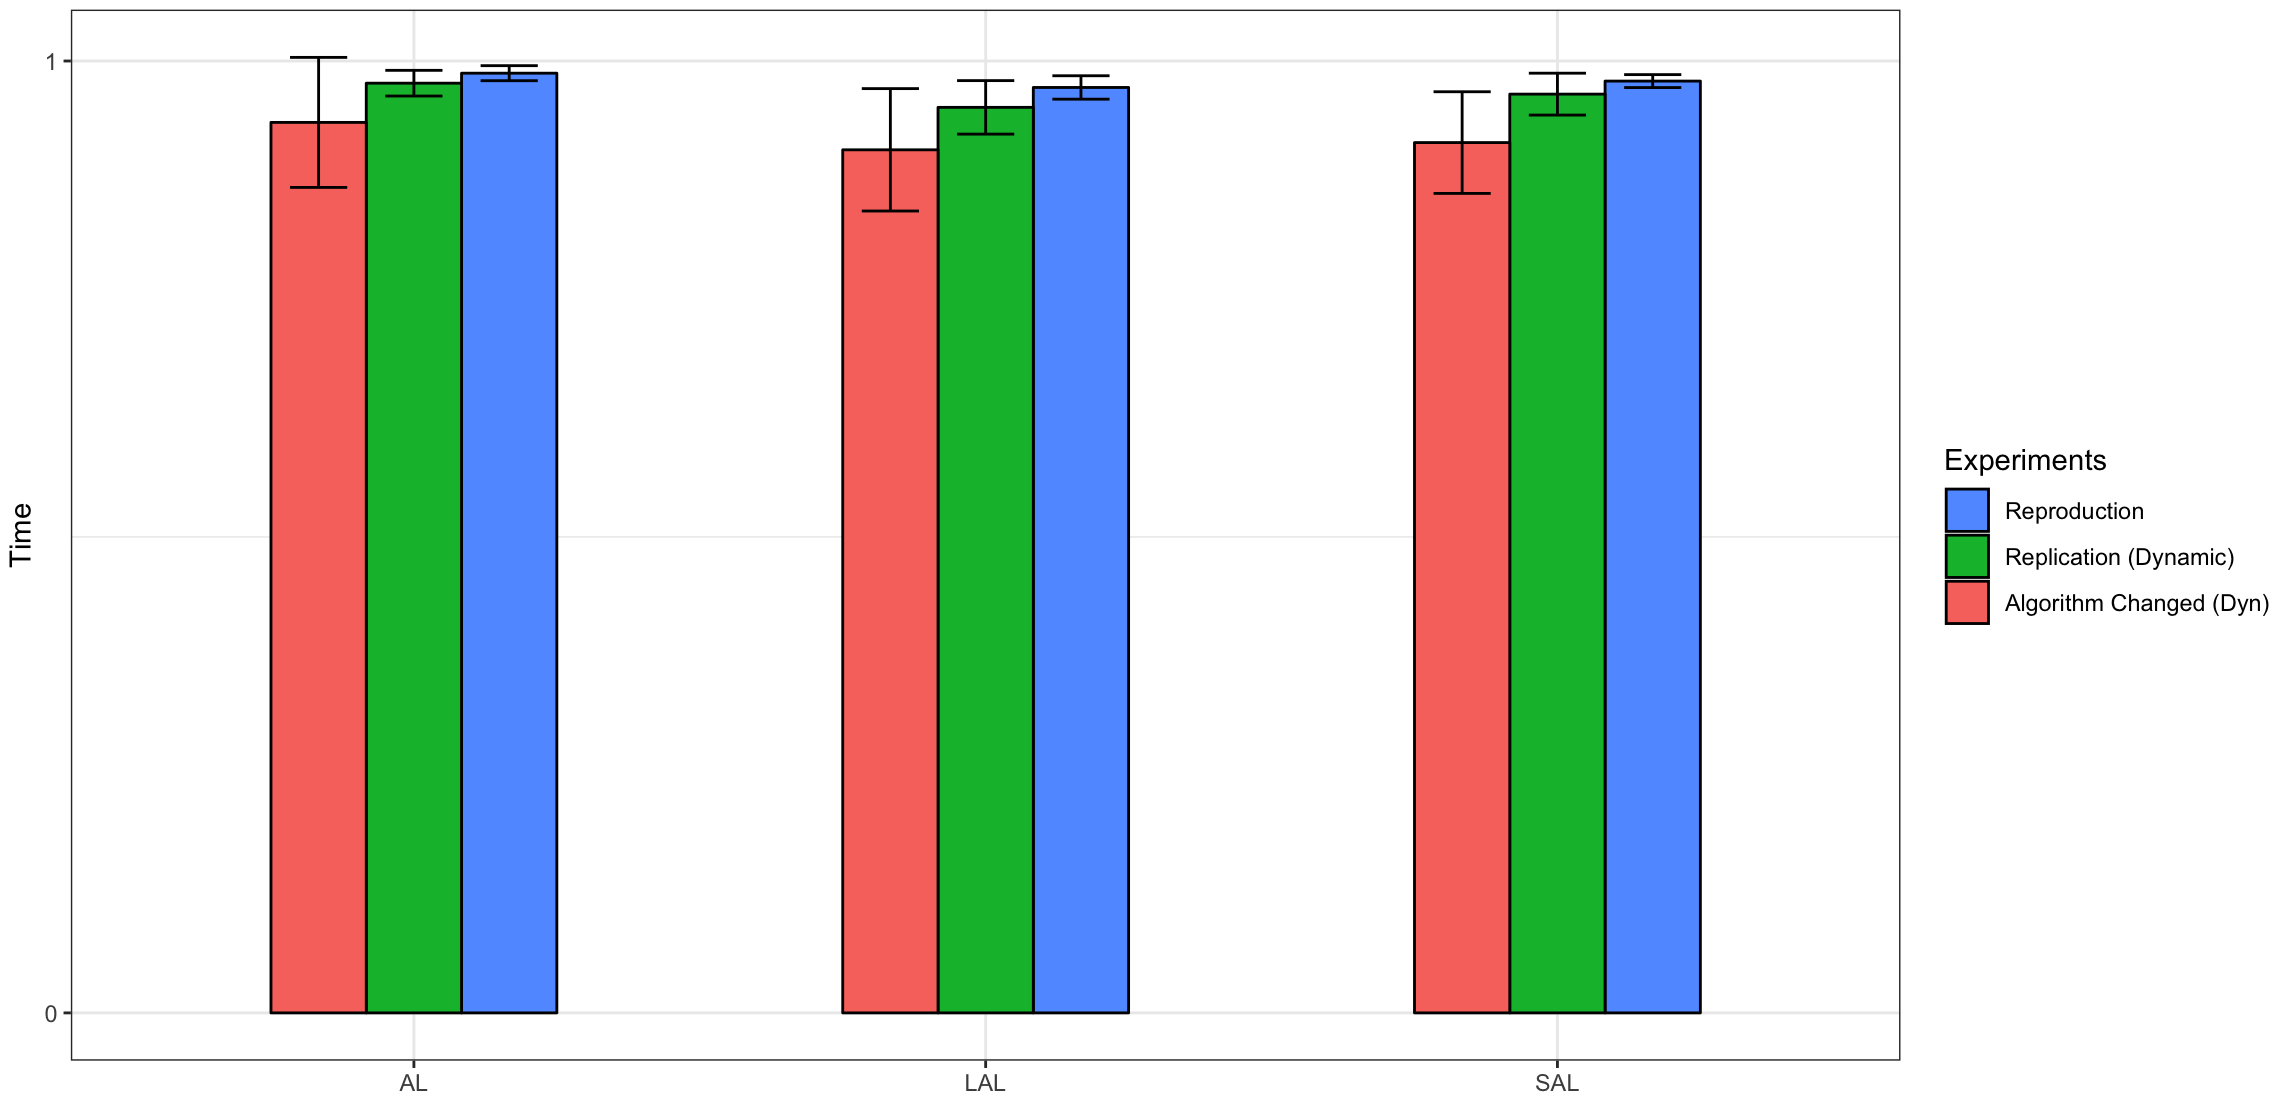
\includegraphics[scale=0.15]{fig/din3.png}
		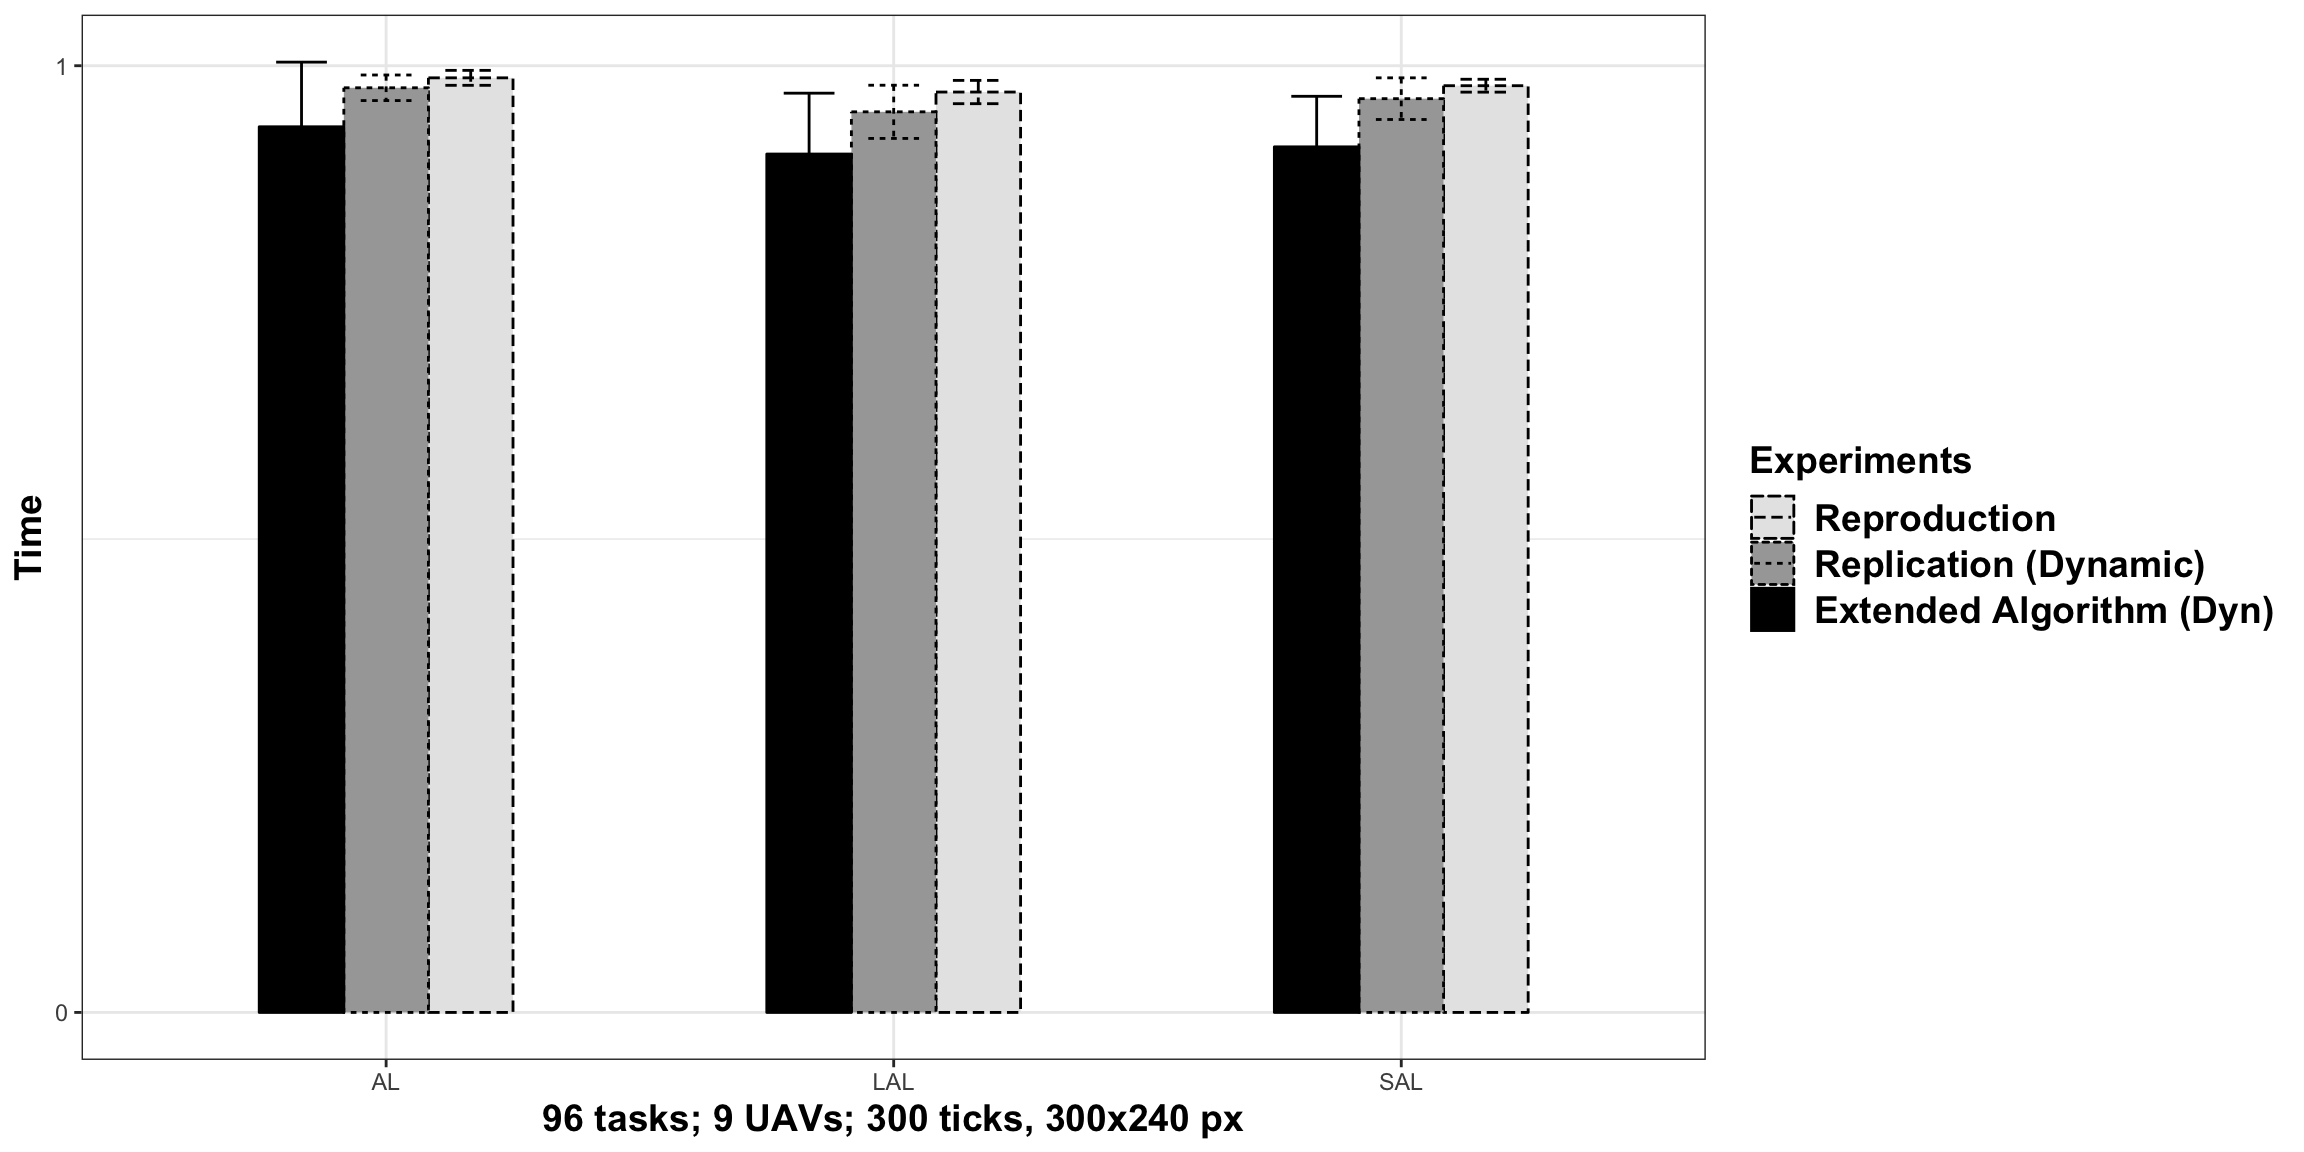
\includegraphics[scale=0.15]{fig/GRAPH08.png}
		\caption{Elapsed Time  in the dynamic scenario (replication) to the original algorithm in static scenario (reproduction), in the dynamic scenario (replication) and the modified ones (96 tasks; 9 UAVs; 300 x 240; 300 ticks)}
		\label{fig:din02}
	\end{center}
\end{figure}

Analyzing the number of finished tasks, depicted in Figure \ref{fig:box01}, it is visible a decrease comparing the algorithms. The lowest one is for the extended algorithms and it occurs because the team spends more time communicating and adjusting the tasks allocation in order to optimize quality thus with less available time for task execution. However, the difference runs into the standard deviation as seen in Figure \ref{fig:box01}.

\begin{figure}[!htb]
\centering
\subfloat{
%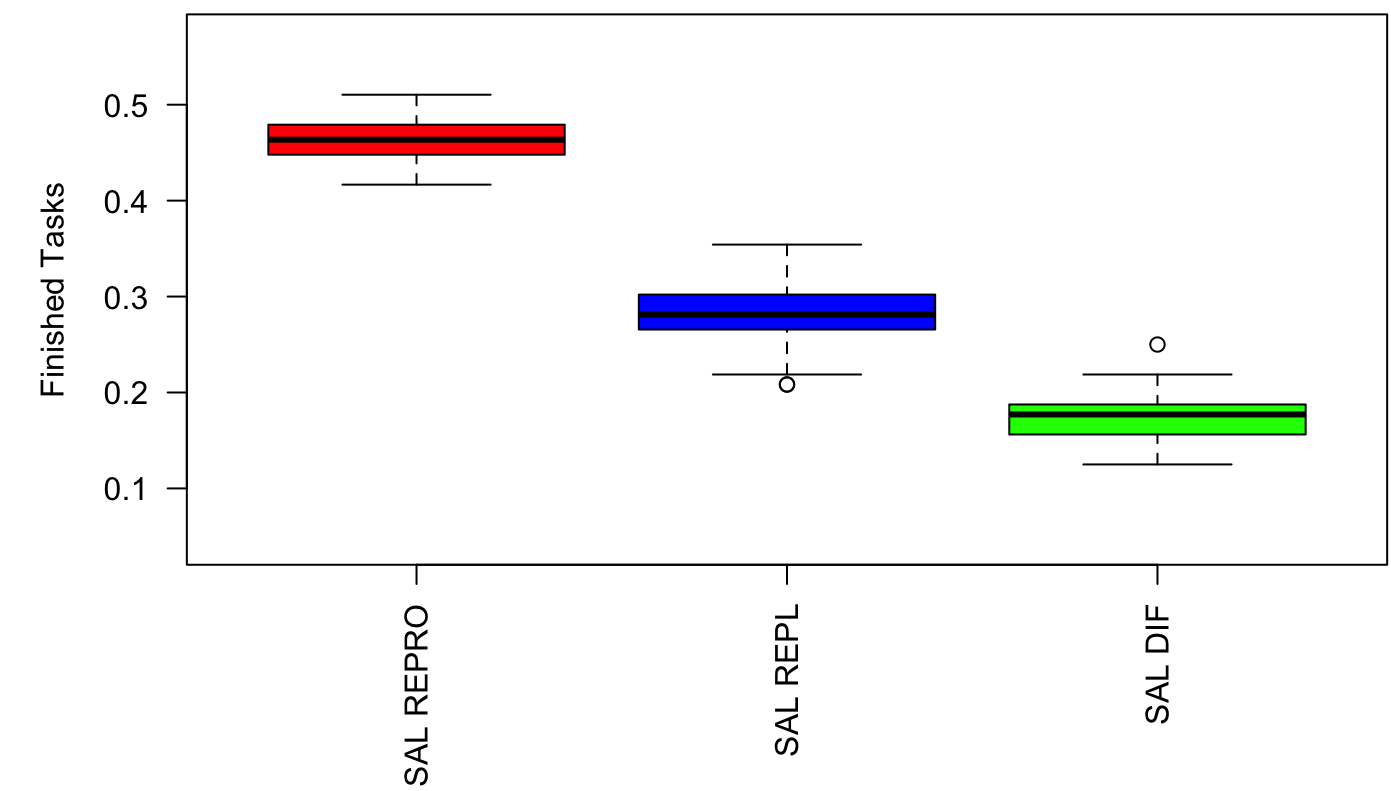
\includegraphics[scale=0.1]{fig/box1.png}
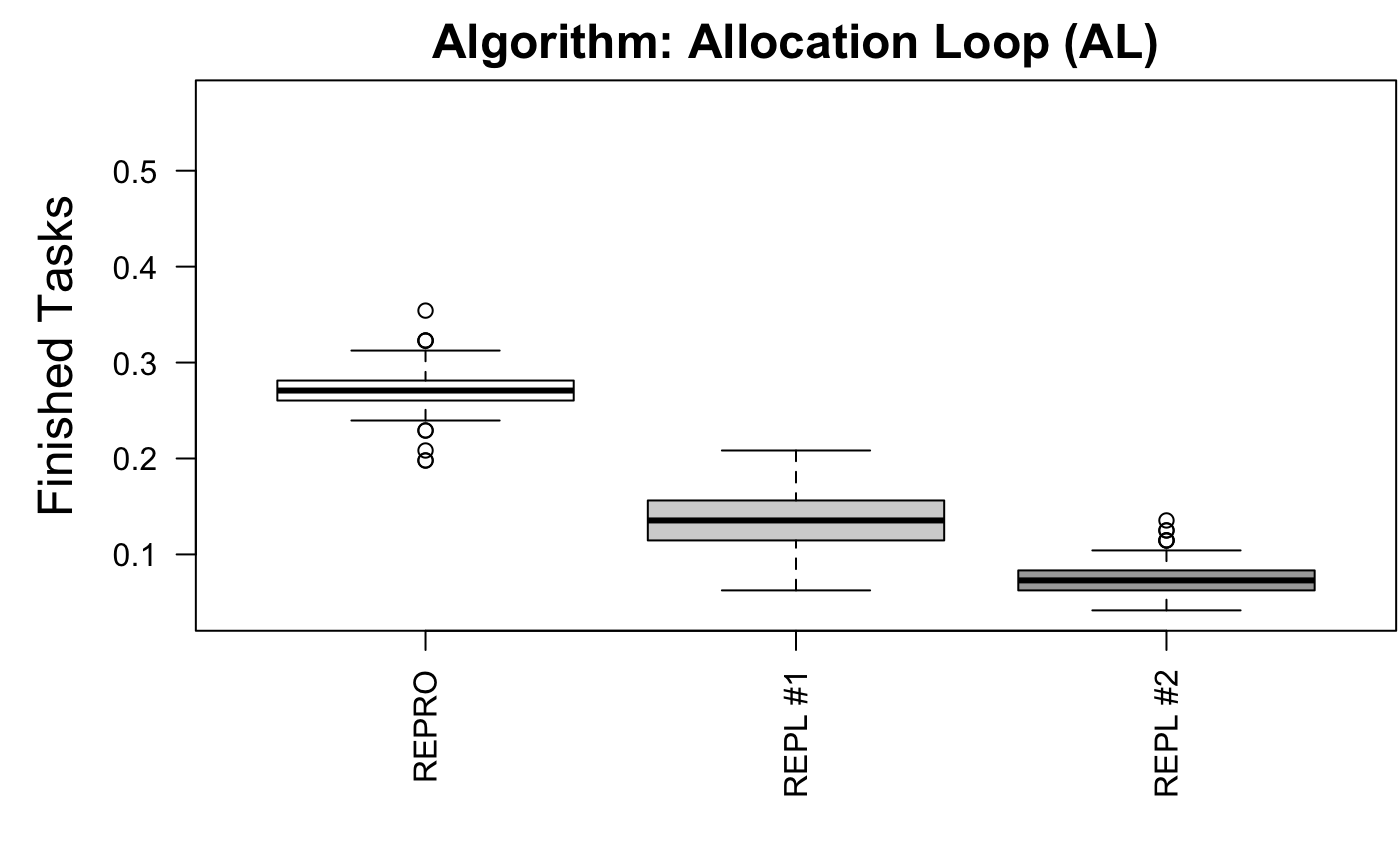
\includegraphics[scale=0.1]{fig/BOX01.png}
}
\quad
\subfloat{
%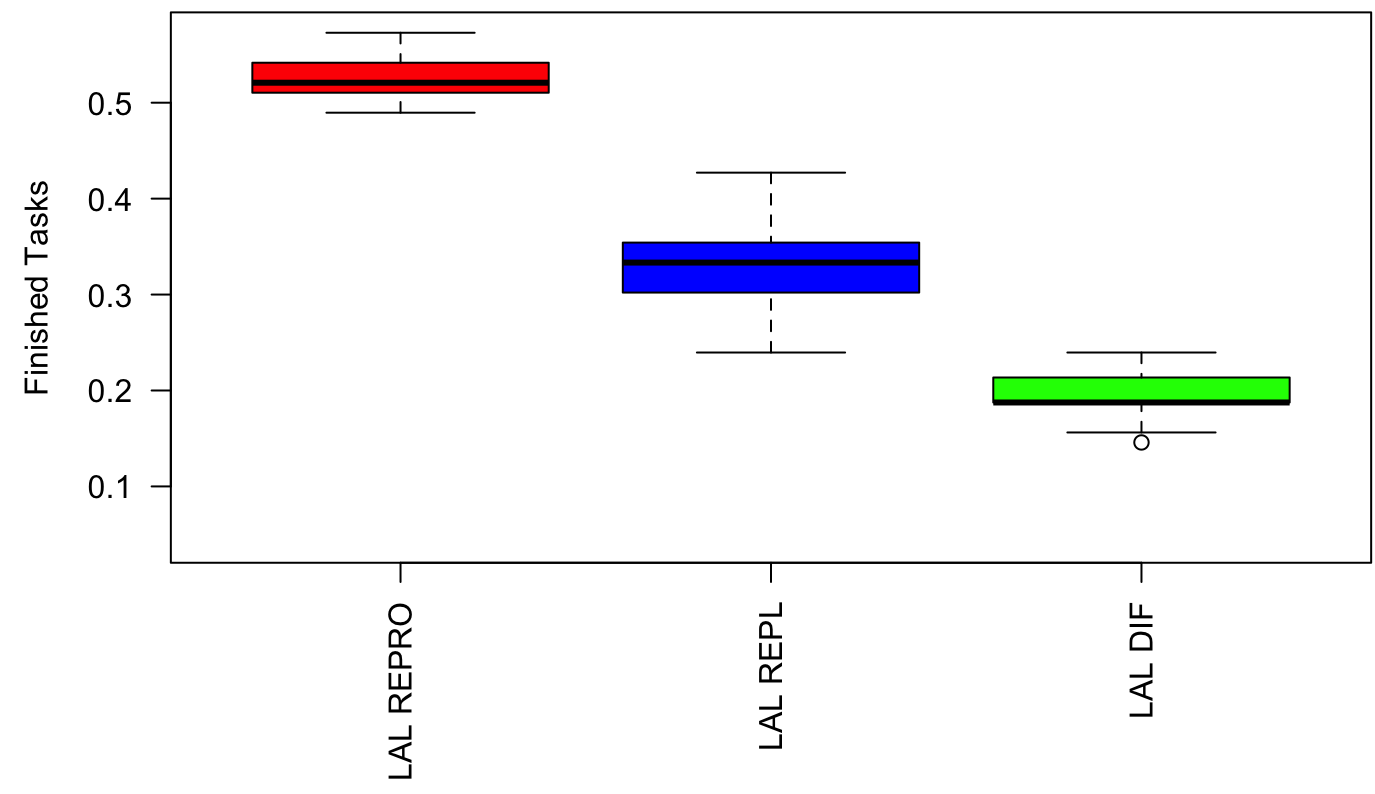
\includegraphics[scale=0.1]{fig/box2.png}
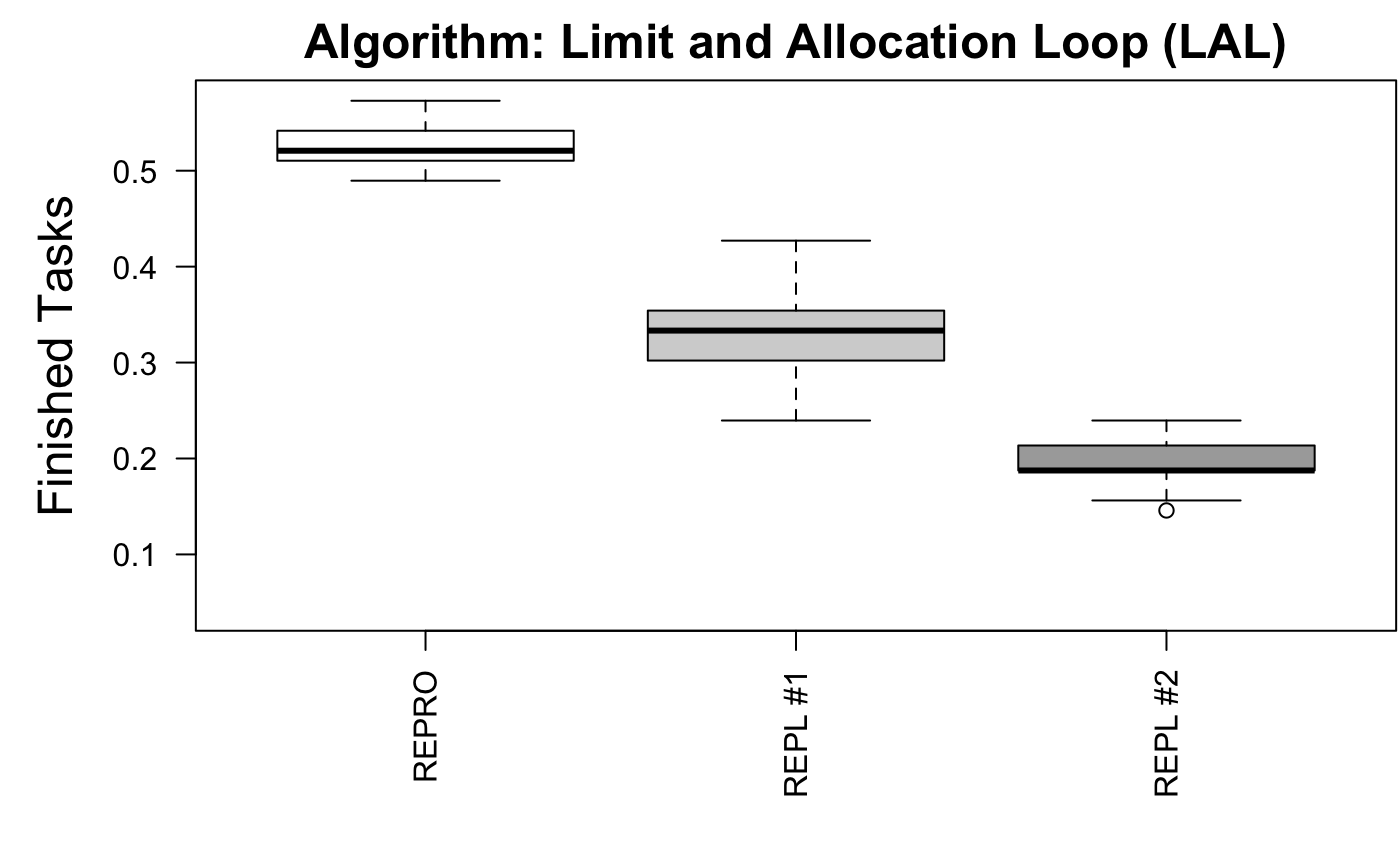
\includegraphics[scale=0.1]{fig/BOX02.png}
}
\quad
\subfloat{
%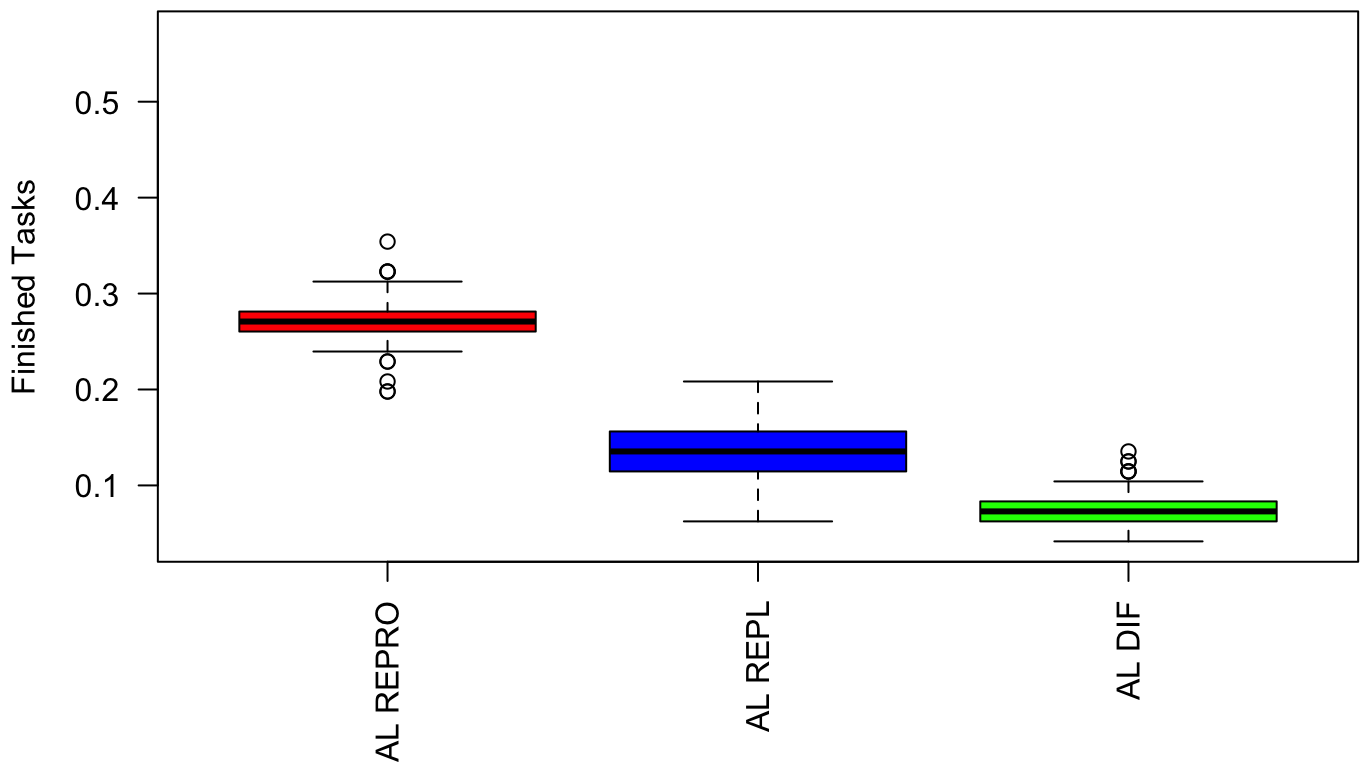
\includegraphics[scale=0.1]{fig/box3.png}
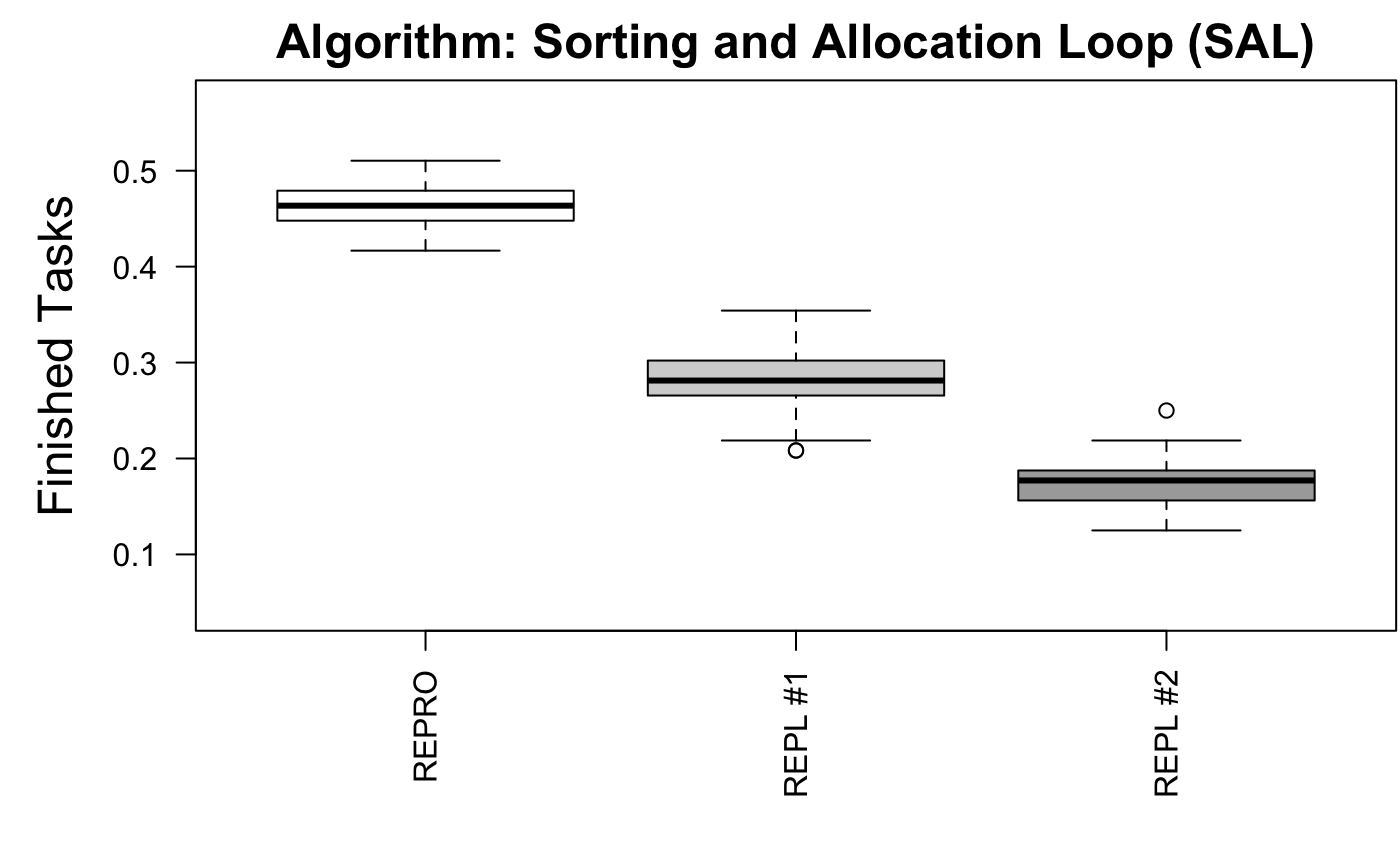
\includegraphics[scale=0.1]{fig/BOX03.png}
}
\caption{Finished tasks to the original algorithm in static scenario (reproduction - REPRO), in the dynamic scenario (first replication - REPL #1) and the extended algorithm in dynamic context (second replication - REPL #2) with the attributes: 96 tasks; 9 UAVs; 300 x 240; 300 ticks and 100 executions}
\label{fig:box01}
\end{figure}

The confirmation of the statistical significance of the difference of such values was obtained by a t-Test, which was employed because the results distribution is close to a normal one, as show in Figure \ref{fig:fig07}. Thus, it is confirmed that the average quality and messages results obtained by the original algorithms and the modified ones are different. The test confirmed the difference with a confidence interval of $0.99$ and $p-val<0.05$. 

\begin{figure}[!htb]
\centering
\subfloat{
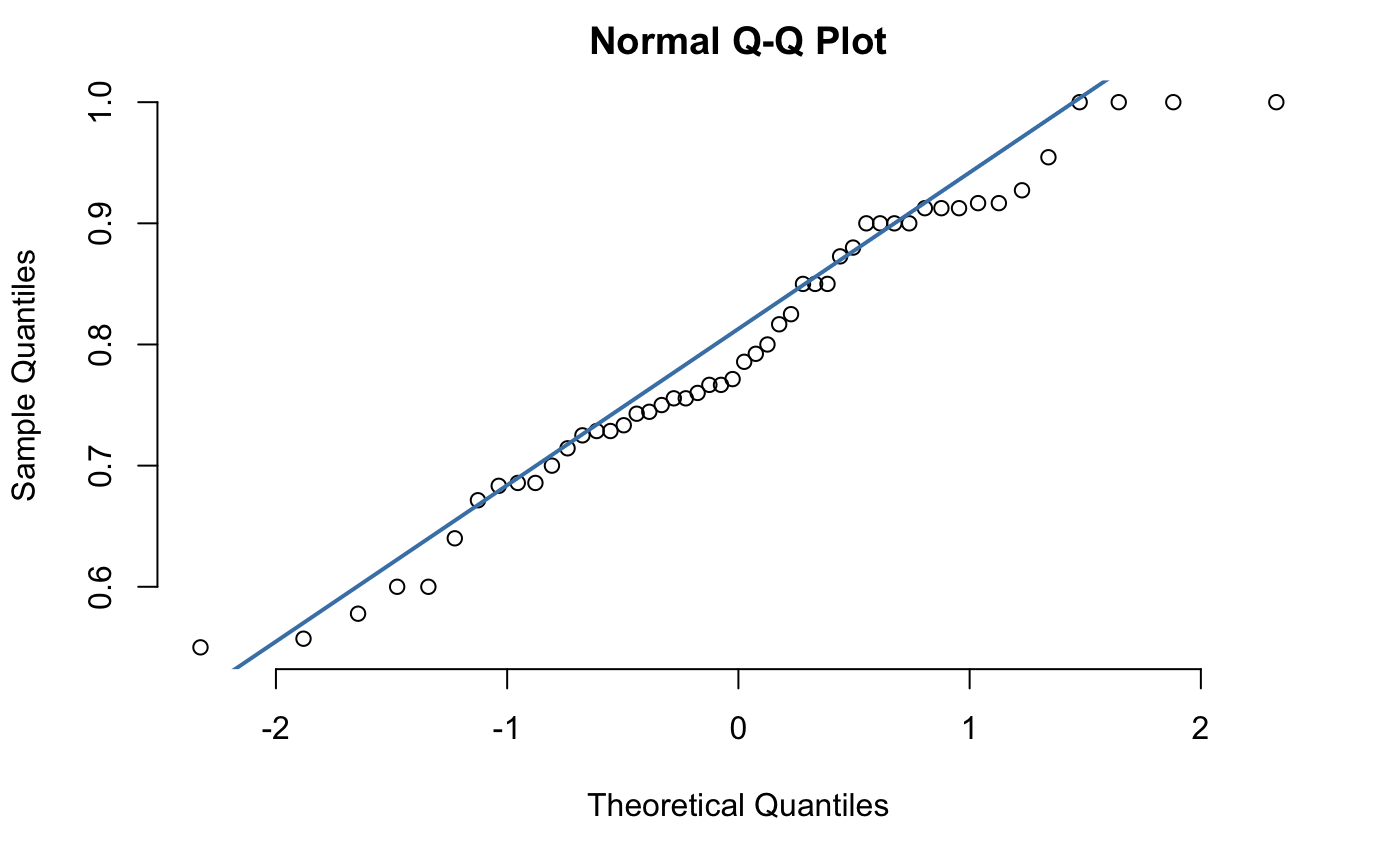
\includegraphics[scale=0.1]{fig/GRAPH09.png}
}
\quad
\subfloat{
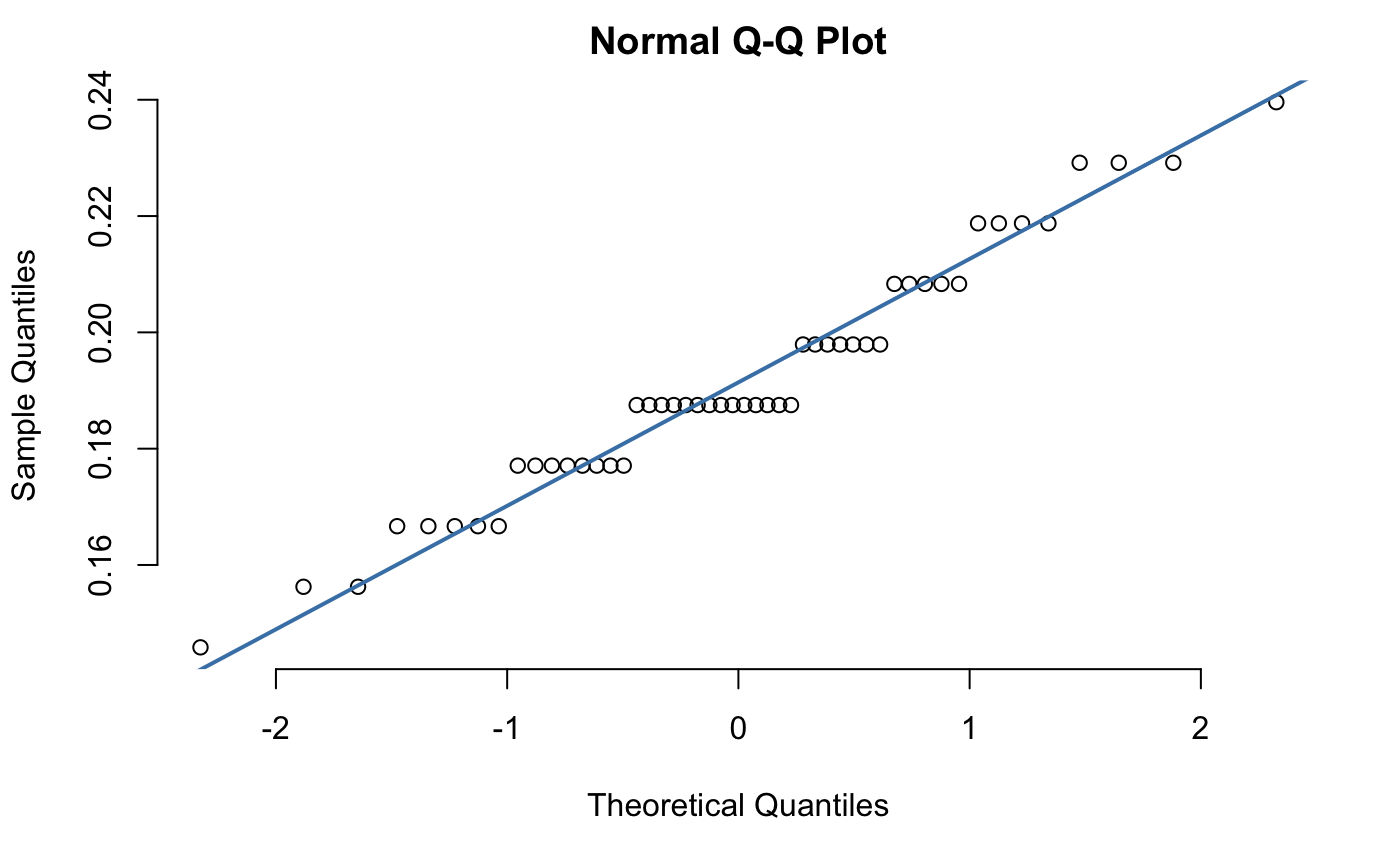
\includegraphics[scale=0.1]{fig/GRAPH10.png}
}
\caption{Distribution of finished tasks (left) and quality (right) results compared with the Normal Graph (Extended SAL algorithm; 96 tasks; 9 UAVs; 300 x 240; 300 ticks; 50 executions)}
\label{fig:fig07}
\end{figure}

For this replication, the $stimulus$ value applied was of $0.6$. It is the same value applied by the original work and the reproduction done in the beginning of the present study (Section \ref{sec:method}). The justification of its use is presented in \cite{MAS07} and \cite{ferreira2007swarm}.

As it was done in Section \ref{sec:original}, different values to the \textit{stimulus} attribute were tested. However, when the results obtained with different \textit{stimulus} values were compared, the variation stayed into the standard deviation. To allow a faithful final comparison in this work, the value used by the original work \cite{MAS07} of $0.6$ was also used to this independent variable (Section \ref{sec:discussion}).
